\documentclass[language=norsk]{ezreport}
\usepackage{lmodern}

% \usepackage[landscape, margin=1.5cm]{geometry}
\usepackage{graphicx}
\usepackage{listings}
\usepackage{lmodern}
\usepackage{norsk}
%\usepackage{fullpage}
%\usepackage[usenames,dvipsnames]{xcolor}	% different hilight colors
%\usepackage{fancyhdr} % used for footer

% used to import title page
\newcommand{\HRule}{\rule{\linewidth}{0.5mm}}


\newcommand{\hilight}[1]{\colorbox{yellow}{#1}}
\newcommand{\hilightblue}[1]{\colorbox{blue}{#1}}


\title{Dokumentasjon: Heisprosjekt}
\author{Sigvart M. Hovland \\
		Olav Kallerud \\
		Gruppe: 39}
\date{\today}

\setlength{\parindent}{0pt}
\setlength{\parskip}{2ex}


\begin{document}

\begin{titlepage}
Dokumentasjon: TTK4125
Datastyring av heis \\
Sigvart M. Hovland \\
Olav Kallerud \\
Gruppe: 39

\begin{center}
\includegraphics[scale=1]{./elevator.png}
\end{center}
\end{titlepage}

\section*{Presisering av produktspesifikasjonen}
\begin{itemize}
	\item{Ved oppstart vil heisen kjøre opp til nærmeste etasje.}
	\item{Ved bestilling forutsetter vi at en bestilling er ''logisk'', med det mener vi at hvis heisen allerede er på vei oppover, prioriteres bestillinger som også skal oppover. Bestillingene blir fortsatt registrert, men tatt til slutt. Som et annet eksempel, hvis en bruker av heisen trykker på ''opp'', men bestiller en etasje ned, så blir bestillingen nedprioritert.}
	\item{Når det ikke er noen bestillinger lukker heisen dørene og blir værende i samme etasje i påvente av nye ordrer.}
	\item{Obstruksjon er kun gyldig når heisen er i en etasje}
\end{itemize}

\section*{Use Case}
\subsection*{Kjør Heis}
\emph{Forutsetning:}\\
Heis i gyldig tilstand; enten i ro i en etasje eller på vei mellom to etasjer.\\\\
\emph{Utløser:}\\
Bestillingsknapp trykkes\\\\
\emph{Suksesscenario}
\begin{enumerate}
	\item{Passasjer bestiller heis}
	\item{Heis starter mot bestilt etasje}
	\item{Heis stopper i ønsket etasje}
	\item{Dør åpnes og passasjer entrer heisvognen}
	\item{Dørene lukkes}
	\item{Bestilling mottas fra passasjer}
	\item{Heis kjører til ønsket destinasjon og stopper der, passasjer går ut av vognen}
	\item{Heis behandler nye bestillinger, returnerer til punkt 2} 
\end{enumerate}
\emph{Utvidelser:}
\begin{itemize} 
	\item[5a]{Obstruksjon i dør}
		\begin{enumerate}
			\item{Dør holdes åpen inntil obstruksjonen er fjernet}
			\item{Hopp til 5}
		\end{enumerate}
	\item[7a]{En passasjer trykker nødstopp}
		\begin{enumerate}
			\item{Heisen stopper}
			\item{Bestillinger slettes}
			\item{Venter på bestilling fra heispanel}
			\item{Hopp til 7}
		\end{enumerate}
	\item[7b]{Det eksisterer en bestilling med høyere prioritet}
		\begin{enumerate}
			\item {Utfør denne bestillingen først} 
			\item {Hopp til 7}
		\end{enumerate}
	\item[8a]{Det ikke er flere bestillinger}
		\begin{enumerate}
			\item{Lukk dør}
			\item{Vent i etasje på ny bestilling}
			\item{Hopp til 7}
		\end{enumerate}
\end{itemize}
\emph{Suksessgaranti}\\
Person ankommer sin ønskede bestilling innen rimelig tid.\\\\
\emph{Minimal garanti}\\
Heis i ro.

\subsection*{Service}
Vi har valgt å ikke utdype service use case siden dette ikke skal implementeres.

\section*{Egenskapsrommet}
For å best mulig beskrive heisens styresystem, har vi valgt å illustrere egenskapsrommets tre dimensjoner ved hjelp av kommunikasjonsdiagram, klassediagram og tilstandsdiagram. 

\includefigure[width=1.0\textwidth]{Strukturdiagram.png}{fig:struktur}{Overordnet strukturdiagram}

\subsection*{Kommunikasjonsrommet: \emph{Kommunikasjonsdiagram}}
\includefigure{kommunikasjonsdiagram.png}{fig:komdia}{Kommunikasjonsdiagram til heismoduler}
\subsubsection*{Control}
Control inneholder tilstandsmaskinen som tar bestemmelser for hva heisen skal gjøre. Den er fullstendig passiv i den forstand at User Interface og Elevator stimulerer tilstandsmaskinen med input (kalt ''events'' i implementasjonen).

\subsubsection*{User Interface}
User Interface registrerer bestillinger fra brukeren, setter respektive indikatorer på panelene og signaliserer til Control at ordre er registrert.

\subsubsection*{Elevator}
Elevator-modulen håndterer det som har med den fysiske heisen å gjøre; gir beskjed til Control når heisen har nådd en etasje, setter etasjeindikator, og setter hastigheten til heismotoren ved beskjed fra Control.

\subsection*{Oppførselsrommet: \emph{Tilstandsdiagram}}
\includefigure{FSM.png}{fig:fsmdia}{Tilstandsmaskin}

\newpage
\section*{Søk etter beste ordre tilgjengelig}
Når Control enheten har fått beskjed om at det finnes ordre, må den beslutte hvilken ordre som er best. Dette avhenger kun av hvor man er og hvilken retning ordren man eventuelt allerede holder på med har. 

Vi har laget en figur som illustrerer vår prioriterte rekkefølge av ordre. Figuren viser en etasje og hvilke type ordre som kan forekomme i hver etasje. En ordre fra inne i heisen gjelder både som ''going down'' og ''going up'' ordre. Prosedyren for å finne en ordre begynner ved å først sjekke i gjeldene etasje etter ordre, deretter følge pilene i den rekkefølgen diagrammet viser. Man begynner i samme retning som den ordren man eventuelt allerede holder på med har, altså hvis man er igang med å transportere noen oppover, søker man videre oppover etter nye ordre. På den måten får man med seg personer som ønsker seg i samme retning.

\includefigure{sok_flyt.png}{fig:sok}{Søkerekkefølge}

\subsection*{Komposisjonsrommet: \emph{Klassediagram}}

\includefigure[width=0.9\textwidth]{klassedia.png}{fig:klassedia}{Klassediagram}

Vi har ikke inkludert I/O-modulen i klassediagrammet, da vi ikke har implementert denne modulen selv. For å beholde oversikten i klassediagrammet har vi valgt å heller ikke inkludere systemets enumerations.

\section*{Kommentarer til implementasjon}
Vi har valgt å kjøre koden flertrådet ved hjelp av ''pthreads'' biblioteket. Grunnen til dette er at det forenklet det å lese input samtidig som man styrer prosessen, men mest brukte vi tråder for å gjøre prosjektet enda litt mer artig. 

Vi har også fokusert mye på modularisering ved å dele opp systemet i moduler som gjenspeiler de fysiske aspektene ved heisen. For ikke å miste oversikten over hvor de ulike funksjonene hører til, har vi gitt dem prefix navnet på modulen. ui\_init() f.eks er da initialiseringsfunksjonen for ui-modulen. På tross av oppdelingen av kode har vi greid oss uten globale variable takket vere get/set-funksjoner og static variable i modulene. Gjennom prosjektet har vi erfart at skikkelig dokumentasjon og planlegging av prosjektet gjør det vesentlig enklere og raskere å gjennomføre selve implementasjonen. Dette gjorde starten av prosjektet veldig grei, men etter hvert som vi kom til ting vi ikke hadde tenkt like nøye gjennom måtte vi revurdere. Moralen er altså at planlegging/dokumentasjon er viktig, men vel så viktig er det å være fleksibel for uforutsette forandringer. Her er en stor fordel med modulær kode.

\section*{V-modellen}
For å sikre en god utviklingsprosess, forsøkte vi å følge den pragmatiske V-modellen. Dette innebar endel testing av de ulike funksjonene underveis ved hjelp av f.eks. modultesting, og test av det overordnede systemet når vi satt det sammen. Testingen vi gjorde underveis har sikret god kontroll på systemets oppførsel og at det gjorde det vi ville og tilfredsstiller kravene som ble stilt i krav spesifikasjonen.

For å sikre god versjonskontroll og utviklings metodikk har vi benyttet oss av versjonskontrollsystemet \emph{git}.

\section*{Modelleringsendringer underveis i prosjektet}
En av de mest synlige endringene i vi har gjort underveis var å splitte opp elev-modulen vi fikk utlevert, og inkludere disse delene User Interface og Elevator. Dette ble gjort for å tydeliggjøre inndelingen av systemet i brukergrensesnitt og heis.

Vi har også fjernet invalid som en tilstand. Invalid er nå bare en for-tilstand der heisen befinner seg før den har blitt initialisert. Resultatet av denne forenklingen var at tilstandsmaskinen i implementasjonen fikk en tilstand mindre og dermed ble enklere, uten at det gikk ut over funksjonaliteten til heisen.

I utgangspunktet hadde vi plassert funksjonen som finner frem til mest gunstige ordre i User Interface, da det er i denne modulen bestillingene blir registrert. Etter nøye ettertanke flyttet vi denne funksjonen til Control, siden det er her alle andre bestemmelser om heisens oppførsel gjøres. Dette bidrar til modulariseringen av koden.

I utvidelsen av produktspesifikasjonen hadde vi først tenkt at heisen skulle kjøre til første etasje etter en viss tid uten bestillinger. Dette har vi revurdert og kommet frem til at det i de fleste tilfeller, særlig i perioder med få bestillinger, vil vere hensiktsmessig å bare la heisen stå i ro i etasjen og vente på nye bestillinger. Dette kan selvsagt tilpasses for den spesifike lokasjonen heisen befinner seg på. For eksempel kan det tidlig på dagen i en kontorbygning vere ønskelig at heisen kjører til inngangsetasjen mens den venter på ordre, da det trolig er mange som skal fra inngangsetasjen til jobb. 

Strukturdiagrammet gir kunden god oversikt over systemet. Gjennom design av dette diagrammet fant vi ut at det også hadde vært greit å ha under implementasjonen. Noterer dette bak øret til neste prosjekt.

%\includefigure{IntegralSinus.jpg}{fig:test}{Dette er en fin forklarende tekst relatert til det inkluderte bildet.}  % Optional: argumenter til includegraphics
%\begin{table}{cccc}{tab:test}{Dette er en informativ tekst angående tabellen.}
%Test & Test & Test & Test \\
%\tablesection
%blah & blah & blah & blah \\
%blah & blah & blah & blah \\
%blah & blah & blah & blah \\
%blah & blah & blah & blah \\
%blah & blah & blah & blah \\
%blah & blah & blah & blah \\
%\tablesection
%blah & blah & blah & blah \\
%blah & blah & blah & blah \\
%blah & blah & blah & blah \\
%blah & blah & blah & blah \\
%blah & blah & blah & blah \\
%blah & blah & blah & blah \\
%\end{table}
%
%\begin{code}{Matlab}{code:test}{Dette er noe eksempeltekst.}
%disp('Hello world!')
%disp('Hello world!')
%disp('Hello world!')
%\end{code}

\section*{UML diagrammer}
\begin{center}
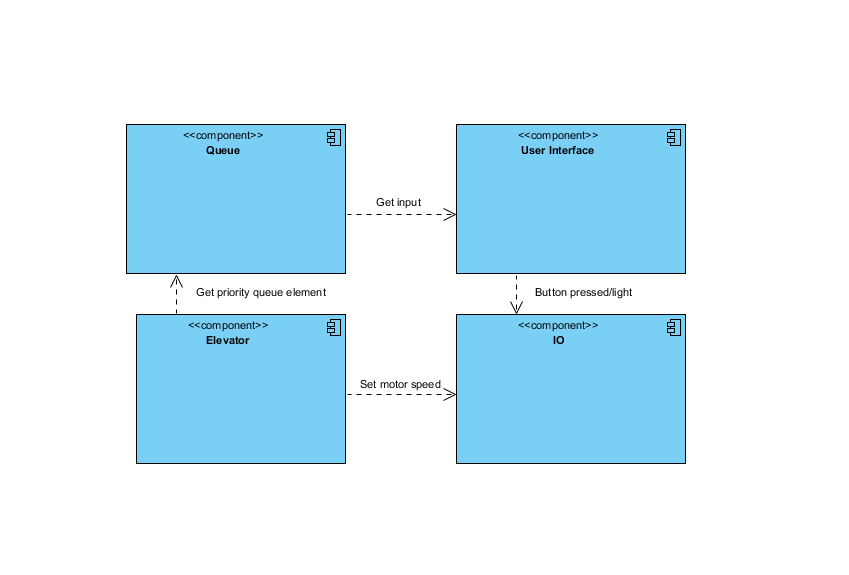
\includegraphics[scale=0.50]{./overordnet_diagram.png}
\\Overordnet kommunikasjons diagram
\end{center}

\begin{center}
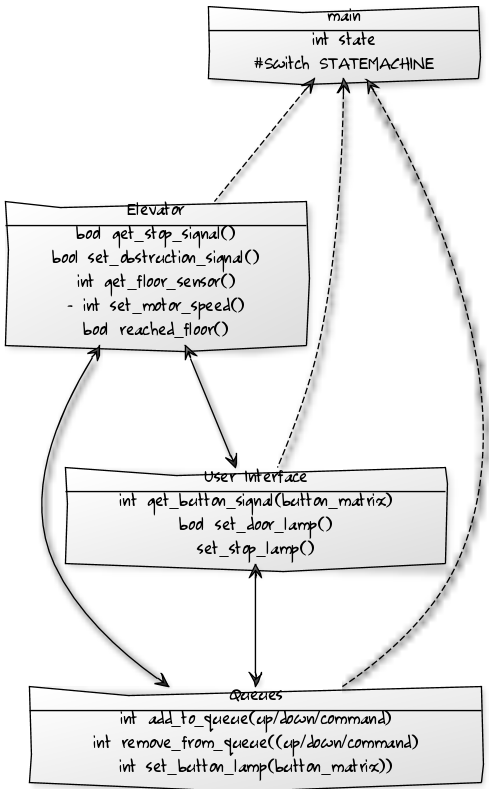
\includegraphics[scale=0.30]{./class_diagram.png}
\\Klasse diagram
\end{center}

\begin{center}
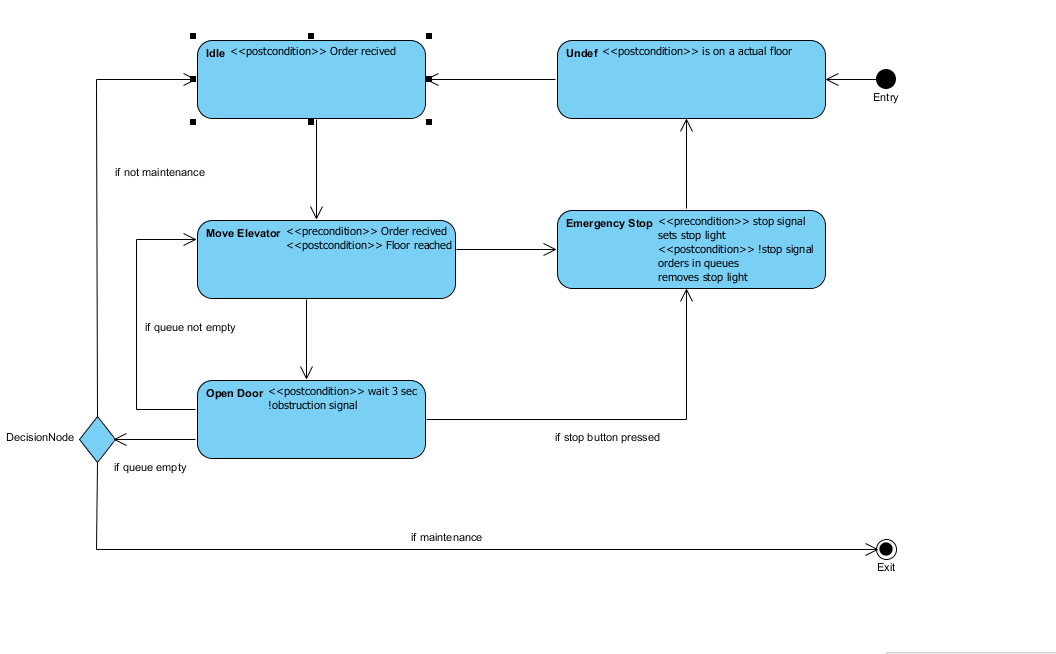
\includegraphics[scale=0.71 angel=90]{./activity_diagram.png}
\\Aktivitetsdiagram
\end{center}

\begin{center}
\includegraphics[scale=0.70,angle=90]{./usecase.png}
\\Use case diagram
\end{center}

\begin{center}
\includegraphics[scale=0.50]{./statediagram.png}
\\Tilstandsdiagram
\end{center}


\end{document}
